\subsection{Recap: How to Implement Features?}
\begin{frame}{\myframetitle}
	\begin{mycolumns}
		\myexampletight{Given a feature model for graphs \ldots}{
			\centering\featureDiagramGraphs
			%\featureDiagramLegend
		}
		\myexample{\ldots\ we can derive a valid configuration}{
			\small
			\leftmiddleandright{
				$\{G\}$\\
				$\{G,C\}$\\
				$\{G,D\}$\\
				$\{G,C,D\}$\\
			}{
				$\{G,W\}$\\
				$\{G,C,W\}$\\
				$\{G,D,W\}$\\
				$\{G,C,D,W\}$\\
			}{
				$\{G,W,S\}$\\
				$\{G,C,W,S\}$\\
				$\{G,D,W,S\}$\\
				$\{G,C,D,W,S\}$\\
			}
		}
	\mynextcolumn		
		\myexampletight{How to Generate Products Automatically?}{
			\centering\foreach \page in {2,12,4,14,6,16,8,18}{\includegraphics[width=.23\linewidth,page=\page]{graphs} }
		}
		\mynote{Goals}{
			\begin{itemize}
				\item Descriptive specification of a product (i.e., a configuration, a selection of features)
				\item Automated generation of a product with compile-time variability
			\end{itemize}			
		}
	\end{mycolumns}
\end{frame}

\begin{frame}{Recap: Features with Build Systems}
	\begin{mycolumns}[widths={40,60},animation=none]
		\myexampletight{}{
			\centering
			\pic[width=.65\linewidth]{pignap-features}
		}
	\mynextcolumn
		\mydefinition{Conditional Compilation with Build Systems}{
			\begin{itemize}
				\item Exploit the expressiveness of a build system's configuration language
				\item In- and exclude individual files or entire directories based on feature selection
			\end{itemize}
		}
		\uncover<2->{\mynote{Major Challenges}{
			\begin{itemize}
				\item Build scripts may become complex, there is no limit to what can be done (e.g., you can run arbitrary shell commands on files)\\
					$\Rightarrow$ \emph{Hard to understand and analyze}
				\item No simple in- and exclusion of individual lines or chunks of code\\
					$\Rightarrow$ High-level use \emph{only}!
			\end{itemize}
		}}
	\end{mycolumns}
\end{frame}

\begin{frame}{Recap: Features with Preprocessors}
	\begin{mycolumns}[widths={40,60},animation=none]
		\myexampletight{}{
			\centering
			\pic[width=\linewidth,page=1,trim=15 20 185 40,clip]{preprocessor-wilderness}
		}
	\mynextcolumn
		\mydefinition{Conditional Compilation with Preprocessors}{
			\begin{itemize}
				\item Use conditional compilation facilities provided by preprocessors 
				\item Annotate and potentially remove code fragments, depending on feature selection
			\end{itemize}
		}
		\uncover<2->{\mynote{Major Challenges}{
			\begin{itemize}
				\item May \emph{obfuscate} source code and severely impact its readability
				\item Hard to analyze and process for existing IDEs
				\item Often used in an ad-hoc or \emph{undisciplined} fashion
				\item Prone to subtle syntax, type, or runtime errors which are hard to detect
				\item \emph{Scattering} and \emph{tangling}\\
					$\Rightarrow$ Separation of concerns?
			\end{itemize}
		}}
	\end{mycolumns}
\end{frame}

\subsection{Modularity}
\begin{frame}{Modularity}
	\begin{mycolumns}[widths={50,50},animation=none]
		\mydefinition{Modularization}{
			Consistent application of \emph{information hiding} and \emph{data encapsulation} to achieve:
			\begin{itemize}
				\item Strong logical connection between the inner parts of a module (high cohesion)
				\item Precisely defined, minimal interfaces (low coupling)
			\end{itemize}						
		}
		\pause
		\mydefinition{Coupling and Cohesion}{
			\begin{itemize}
				\item \emph{Cohesion}: Measure of how well the parts of a module work together (intra-module communication).
				\item \emph{Coupling}: Measure of the complexity of inter-module communication (through interfaces).
			\end{itemize}
		}		
	\mynextcolumn
		\vspace{-1cm}
		\myexampletight{High Coupling, Low Cohesion}{
			\centering
			\pic[width=0.5\textwidth]{cohesion_coupling_1}
		}
		\myexampletight{Low Coupling, High Cohesion}{
			\centering
			\pic[width=0.5\textwidth]{cohesion_coupling_2}
		}
	\end{mycolumns}
	\begin{mycolumns}[widths={50,50},animation=none]	
	\end{mycolumns}
\end{frame}

\begin{frame}{Why Modularity?}
	\begin{mycolumns}[widths={45,55},animation=none]
		\mynote{Traditional Reasons}{			
			\begin{itemize}
				\item Modules can be developed independently of each other (collaborative work)
				\item Easier to maintain because changes can be made locally
				\item Data encapsulation promotes stability and reliability
				\item Software is easier to understand:
				\item Hiding complexity behind interfaces
				\item Modular decomposition = divide and conquer
			\end{itemize}						
		}
		\pause
	\mynextcolumn
		\mynote{Modularization and Software Product Lines}{
			\begin{itemize}
				\item \emph{Reuse}: Parts of the software can be {\em reused} 
				\item \emph{Alternatives}: Modules can be {\em exchanged by alternative implementations}
				\item \emph{Variability}: Modules can be {\em reassembled in a new context} (e.g., in other projects)
			\end{itemize}
		}
		\myexampletight{}{
			\pic[width=\linewidth,page=18,trim=5 115 5 5,clip]{lego} 
		}
	\end{mycolumns}	
\end{frame}

\subsection{Software Components}
\begin{frame}{Components}
	\begin{mycolumns}[widths={50,50},animation=none]
		\mydefinition{Component \mysource{\szyperski}}{			
			A software component is a unit of composition with contractually specified \emph{interfaces} and explicit \emph{context dependencies} only. 
			A software component can be deployed independently and is \emph{subject to composition} by third parties.
		}
		\myexampletight{}{
			\centering
			\pic[width=.7\linewidth]{component_uml.png}
		}	
		\mynote{}{			
			\begin{itemize}
				\item Context/deployment dependencies: Typically container or middleware (e.g., JavaEE, CORBA, OSGi, etc.)
			\end{itemize}
		}
	\mynextcolumn
		\vspace{-0.7cm}
		\mynote{Composition and Reuse: Components}{
			\begin{itemize}
				\item Are composed with other components to form software systems,
				\item Are supposed to be re-usable in other software systems,
				\item May stem from third-party vendors (make-or-buy-decisions, markets for components).
			\end{itemize}			
		}
		\pause
		\myexampletight{UML Component Diagrams}{
			\centering
			\pic[width=\linewidth]{component_diagram_uml.png}
		}
		\pause
	\end{mycolumns}	
\end{frame}

\subsection{Components vs. Objects/Classes}
\begin{frame}{Components vs. Objects/Classes}
	\begin{mycolumns}[widths={40,60},animation=none]
		\mynote{Commonalities}{			
			Lots of similar principles, particularly 
			\begin{itemize}
				\item encapsulation and information hiding,  
				\item accessibility through public interfaces,
				\item (de-)composition and nested objects/components,
				\item etc.				
			\end{itemize}
		}
		\pause
	\mynextcolumn
		\mynote{Differences}{
			\begin{itemize}
				\item \emph{Objects are smaller} than components by focusing on detailed implementation problems (components aim at abstracting from implementation details).
				\item \emph{Object are less cohesive and stronger coupled} than components due to (deliberately) delegating lots of responsibilities to other objects, while components aim at maximizing cohesion and minimizing coupling.
				\item \emph{Objects/classes are reused through inheritance and polymorphism}, while components are reused by being integrated into a component architecture.		
			\end{itemize}			
		}
	\end{mycolumns}	
\end{frame}

\begin{frame}[fragile]{Example: A Color Component \mytitlesource{\fospl}}
	\begin{mycolumns}[columns=2,widths={40,60}]
			\myexample{A Reusable Component}{
				\begin{itemize}
					\item Assume that storing and printing colors is non-trivial (e.g., in our graph library). 
					\item Implement color management as a reusable component, using Java's visibility mechanism to enforce encapsulation.						
				\end{itemize}
			}
		\mynextcolumn
{\small
\begin{codetight}{}
package components.color;

~// public interface~
public class ColorComponent {
	public Color createColor(int r, int g, int b) { ~/* ... /*~ }
	public void printColor(Color color) { ~/* ... /*~ }
	public void mapColor(Object o, Color c) { ~/* ... /*~ }
	public Color getColor(Object o) { ~/* ... /*~ }
	
	~// just one component instance~
	public static ColorComponent getInstance() { return instance; }
	private static ColorComponent instance = new ColorComponent();
	private ColorComponent() { super(); }
}
public interface Color { ~/* ... /*~ }

~// hidden implementation~
class ColorImpl implements Color { ~/* ... /*~ }
class ColorPrinter { ~/* ... /*~ }
class ColorMapping { ~/* ... /*~ }
\end{codetight}
}
	\end{mycolumns}
\end{frame}

\begin{frame}[fragile]{Example: A Color Component}
	\begin{mycolumns}[columns=2,widths={60,40},animation=none]
{\small
\begin{codetight}{}
public class Graph {
	private List<Node> nodes = new ArrayList<Node>();
	public Node add() {
		Node n = null;
		@if (Config.COLORED) {
			Color c = ColorComponent.getInstance().createColor(0, 0, 0);
			n = new Node(nodes.size(), c);
		} else @ {
			n = new Node(nodes.size());
		}
		nodes.add(n);
		return n;
	}
	~// ...~
}
\end{codetight}
}
		\mynextcolumn
\vspace{-0.5cm}
{\small
\begin{codetight}{}
public class Node {
	private int id;
	@private ColorComponent colorComp =
		ColorComponent.getInstance();@
	public Node(int id) { this.id = id; }
	public Node(int id, @Color c@) {
		this(id);
		@colorComp.mapColor(this, c);@
	}
	public void print() {
		@if (Config.COLORED) {
			Color c = colorComp.getColor(this);
			colorComp.printColor(c);
		}@
		System.out.print(id);
	}
}
\end{codetight}
}			
	\end{mycolumns}
	\mynote{}{
		\begin{itemize}
			\item We can \emph{reuse} the Color Component when implementing the color feature for the graph library (but also for other applications). 
			\item However, we need to write custom code to ``connect'' our implementation with the component.\\
				$\Rightarrow$ \emph{Glue Code}
		\end{itemize}
	}
\end{frame}

\subsection{Implementation of Product Lines}
\begin{frame}{Component-Based Implementation of Software Product Lines}
	\begin{mycolumns}[widths={40,60}]
		\mydefinition{General Idea}{					
			\begin{itemize}
				\item Every feature is implemented by a dedicated component.
				\item Feature selection determines which components shall be integrated to form an application.				
			\end{itemize}
		}
		\myexample{Vision}{
			\pic[width=.38\linewidth,height=1.75cm]{lego_components} 
				\vspace*{\fill}
					$\Longrightarrow$ 
				\vspace*{\fill}	
			\pic[width=.47\linewidth,height=1.75cm]{lego_product}
		}
	\mynextcolumn
		\myexample{Reality}{
			\pic[width=.27\linewidth,height=1.75cm]{lego_components} 
				\vspace*{\fill}
					$+$ 
				\vspace*{\fill}	
			\pic[width=.27\linewidth,height=1.75cm]{lego_glue}
				\vspace*{\fill}
					$=$ 
				\vspace*{\fill}	
			\pic[width=.35\linewidth,height=1.75cm]{lego_product}
		}			
		\mynote{Glue Code and Customization}{
			\begin{itemize}
				\item Developers must connect components through glue code (exception: If components are only exchanged against alternative components)
				\item Components may contain run-time variability (e.g., color manager in our example may be parameterized by color model (RGB, CMYK, ...))
			\end{itemize}
		}
	\end{mycolumns}	
\end{frame}

\subsection{The Library Scaling Problem}
\begin{frame}{The Library Scaling Problem}
	\begin{mycolumns}[widths={40,60},animation=none]
		\myexampletight{Decomposition \& Reuse}{
			\centering
			\pic[width=.95\linewidth]{tangram}
		}
	\mynextcolumn
		\mydefinition{What is the optimal size of a component?}{
			\begin{itemize}
				\item Large components (vertical scaling): Typically not widely reusable
				\item Small components (horizontal scaling): Limited payoff for component integrators
			\end{itemize}
		}
		\pause
		\mynote{Practical Compromise}{
			\begin{itemize}
				\item Mostly vertically scaled (i.e., high payoff) components within a few important, narrow domains (e.g., user interface construction systems).
				\item In other words: There is no general market for arbitrary components, but a few specialized market segments.
			\end{itemize}
		}
	\end{mycolumns}
\end{frame}